

\section{General Job Shop Manufacturing Systems}
\label{sec:general-job-shop}

Perhaps the term `class' needs some clarification. A network with a
single class of jobs means that the all jobs have the same service
distribution. In multi-class networks jobs of different classes
typically have different service distributions. Note that we do not
discuss multi-class queueing networks in this course.


\paragraph{Example}

Company X produces paint according to a make-to-stock strategy. It
makes paint in two steps: mixing and filling/packaging. In the first
step, the ingredients are mixed in large vessels. Once mixed, the
vessels are moved to an intermediate stocking point. Here the paint
waits (in the vessels) until the planner decides to package the paint
into cans. Company X has two filling/packaging machines: machine A
fills small, 1 liter cans; machine B fills large, 5 liter cans. Jobs
for machine A (B) line up in front of machine A (B), i.e., each
machine has its own queue, c.f. Figure~\ref{fig:paint}. The paint shop
has 8 hours available per day, and any unfinished work at the end of a
day is carried over to the next working day. The problem of Company X
is that the amount of intermediate stock in queue is too high. This
not only costs money (paint is quite expensive), but also makes
due-date quotation to customers difficult (recall, by Little's law, if
queues are long, waiting times are typically also long).


\begin{figure}[ht]
    \centering
    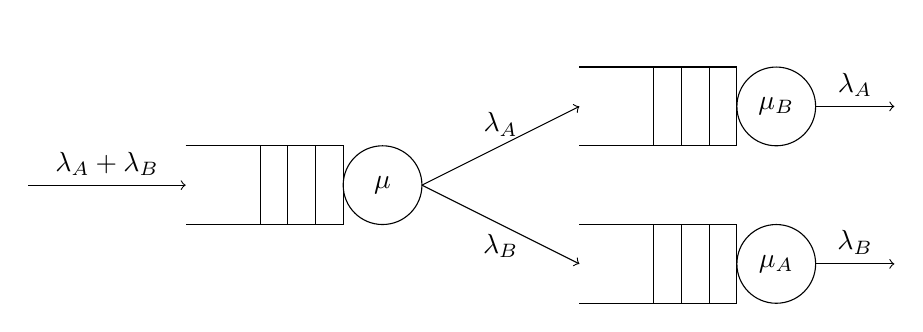
\begin{tikzpicture}[
->-/.style={decoration={markings, mark=at position .5 with {\arrow{stealth}}},
postaction={decorate}},
queuei/.pic={
  \draw%[line width=1pt]
    (0,-0.5) -- ++(2cm,0) -- ++(0,-1cm) -- ++(-2cm,0);
   \foreach \Val in {1,...,3}
     \draw ([xshift=-\Val*10pt]2cm,-0.5) -- ++(0,-1cm);
\draw (2.5,-1) circle [radius=0.5cm] node {#1};}
]
\path 
  (0,0) pic {queuei=$\mu$}
  (5,-1) pic {queuei=$\mu_A$}
  (5,1) pic {queuei=$\mu_B$};

\draw[->] (-2,-1)--(0,-1) node[midway, anchor=south] {$\lambda_A+\lambda_B$};
\draw[->] (3,-1)--(5,0) node[midway,above] {$\lambda_A$}; 
\draw[->] (3,-1)--(5,-2) node[midway,below] {$\lambda_B$}; 
\draw[->] (8,0)--(9,0) node[midway,above] {$\lambda_A$}; 
\draw[->] (8,-2)--(9,-2) node[midway,above] {$\lambda_B$}; 
%\draw[->-] (2.5,-0.5)-- ++(0,-1) -- ++(5.,0) -- ++(0, 1.5); 

\end{tikzpicture}
\caption{A queueing model of a paint factory.}
\label{fig:paint}
\end{figure}

To analyze how to control the average cycle time of an arbitrary job,
whether it is an A or a B job, we can use at least three models.
\begin{enumerate}
\item Model 1. Model all stations as $M/M/1$ queues. As, by
  assumption, the mixing station is an $M/M/1$ queue, its departure
  process is exponential with rate $\lambda_A + \lambda_B$, and of
  these departures, the type A jobs go to filling station A. Thus, we
  can compute the waiting times at stations $A$ and $B$ also. Finally,
  the average waiting time is given by the weighted average of the
  waiting times of the A and B jobs. One weak point of this model is
  the assumption of the exponentiality of the processing times at all
  stations. The data obtained at the paint factory tells that
  processing times are not really exponential.  However, we can model
  the processing times as expoential, and use the ideas of Section
  2.2. of Zijm's book to compute the waiting times.
\item Model 2. Model the second processing step as \emph{one} filling
  station, i.e., put an imaginary box around both filling stations A
  and B, and model it as one station with \emph{one} machine, but such
  that the capacity of this one machine is equal to the capacity of
  the two original filling machines. This is a simple model, but it
  approximates the two filling machines by one machine, and we know
  that multi-server queueing systems behave a bit different from
  single-server queueing systems. Besides that, there are two queues
  in front of the machines, but in this model we merge both queues
  into one.
\item Model 3. Model the second processing step as \emph{one} filling
  station, i.e., put an imaginary box around both filling stations A
  and B, but now model it as one station with \emph{two identical}
  machines.  This is also a simple model, but for this to work we need
  to assume that both machines have the same capacity, i.e.,
  processing speed. This assumption, however, is not satisfied in the
  paint factory.
\end{enumerate}

We see that all three models capture part of the real production
system, but they are also partly wrong.  To analyze the case it is
perhaps best to implement all three models and investigate to what
extent these models give similar or dissimilar results. Once we know
which models appears to give the most realistic, or robust, results,
we can use the models to obtain insight into the situation and provide
ideas how and where to improve the situation. Mind that in general it
is quite pointless to make very detailed models: often only gross data
is available, the data needed to estimate the parameters of
fine-grained models is simply not available, or need to be guesses.
As a conclusion, the analysis of real situation often requires several
models, each with their own strengths and weaknesses.


\begin{question}
  It is mentioned in the text that there are $5M+M^2$ input parameters
  required to characterize an $M$ station network of $G/G/1$ queues. What are these parameters?
  \hint{ Check the formulas in the synthesis carefully.}
  \begin{solution}
    \begin{enumerate}
    \item The routing matrix $P$ is $M$ times $M$, hence contains
      $M^2$ parameters, but often most of them will be zero.
    \item $\lambda_{0i}$ is the arrival rate of external jobs to station $i$, hence $M$ parameters.
    \item $C_{0i}^2$ is the SCV of the interarrival times at station
      $i$, hence $M$ parameters.
    \item $C_{si}^2$ is the SCV of the service times at station $i$,
      hence $M$ parameters.
    \item The expected service times $\E S_i$ at station $i$, 
      hence $M$ parameters.
    \item The number of servers $c_i$ at station $i$, hence $M$
      parameters.
    \end{enumerate}
  \end{solution}
\end{question}



\begin{question}[use=false]
  In this question we develop a simple model to analyze the sojourn
  time at a large pancake restaurant. The restaurant has three large
  dining rooms and a terrace. One a busy summer days there can be more
  than 600 customers present at the same time. The kitchen has a stove
  with 12 burners to make pancakes. Baking one pancake takes about 2
  minutes. One out of five pancakes get an extra topping after
  baking. The chef bakes the pancakes, the assistant handles the
  toppings. We model this situation as a two-station queueing system:
  the chef is the server at the first station, the assistant is the
  server at the second station. The chef is a bit clumsy with his
  tools: about 10\% of the pancakes falls on the floor, hence needs to
  be baked again.  We want to compute the throughput time, i.e, the
  total sojourn time, for this system.

  \begin{enumerate}
  \item Suppose we would model the stove as a $M/M/1$ queueing system
    in which the (single) server works at twelve times the rate of the
    one of the burners. Would this be a good model? 
  \item What is the routing matrix for this queueing system?
\item What is the vector $\vec \gamma$ of external arrivals?
\item Can you find an approximation for the net arrival rate
  $\lambda_1$ and $\lambda_2$ at the two stations? 
  \end{enumerate}


  Up to now we have not yet discussed an important detail, the
  distribution of the inter departure times at the chef. 

  \begin{enumerate}[resume]
  \item Why is this departure process most probably not Poisson?
  \item What type of $C_a^2$ do you expect to see at the assistant? 
  \item How would you estimate the waiting time at the assistant?
  \item Estimate the arrival rate $\alpha$, and compute the utilization of  the chef.
  \item What formula would you use to estimate the average waiting time at the chef?
  \end{enumerate}

    \begin{solution}
      \begin{enumerate}
      \item 
      No, not really, it takes 2 minutes to bake a pancake, no matter
      the amount of burners available.  Thus, only when the queues are
      really long, the difference in sojourn time between a fast single server and multiple, parallel, slow servers would be small. 
    \item   The chef drops 10\% of the pancakes. These have to be re-baked. Of
  the remaining 90\% of the pancakes one out five gets a topping,
  thus, $0.9\cdot0.2=0.18$ goes to the assistant. The assistant
  delivers quality work, so no pancakes have to be processed by him
  again. Thus,
\begin{equation*} 
P=
  \begin{pmatrix}
    1/10 & 9/50 \\
0 & 0
  \end{pmatrix}
\end{equation*}
\item Only the chef gets new orders.  $\vec \gamma = (\alpha, 0)$,
where  $\alpha$ is the arrival rate of new orders.
\item The assistant receives
  20\% of all pancakes: $\lambda_2 = \alpha/5$.  As the chef has to
  redo 10\% of the pancakes, $\lambda_1 = \frac{10}{9}\alpha$.

  We can also solve $\vec \gamma + \vec \lambda P = \vec \lambda$.
  This gives, $\lambda_1 = \alpha + \lambda_1/10$, and
  $\lambda_2 = 9/50 \lambda_1$. Solving this gives the same answers.
\item       The baking of a pancake takes about 2 minutes, and it quite
      regular. Thus, the queueing situation at the chef resembles the
      $M/D/12$ queue. However, due to the rework, there is more variability than in the $M/D/12$ queue. 
    \item       I would guess it would be smaller than 1. By how much is not so
      easy to say. Simulation of the $M/D/12$ queue would be most helpful here.
    \item       As both  $C_a^2$ and $C_s^2$ at the second station are smaller than 1, in particular $C_s^2$ must be quite a bit smaller than 1, I would use the formula:
\begin{equation*}
  \E W_Q \approx \frac{C_a^2 + C_s^2}2 \frac \rho{1-\rho} ES_2,
\end{equation*}
where $\rho=\lambda_2E(S_2)$.
\item       Lets concentrate on a busy day. There are 600 people
      present. Assume they stay one hour on average. By Little's law
      we see that the arrival rate of people is $600/60=10$ per
      minute. Assume half of the people order a pancake, then $\alpha=5$ per minute. As the average baking time is 2 minutes, $\rho = \lambda_1 \E S_1/12 = 5\cdot 10/9\cdot 2/12= 25/27$.
Realize that $\rho=\lambda\E S_1/12$ is not OK. 
\item Since we have many customers, independently arriving and ordering pancakes, it is reasonable to model the arrival process as a Poisson process. Thus, as an approximation
  \begin{equation*}
    \E W_Q \approx \frac12 \frac{\rho^{\sqrt{2(12+1)} - 1}}{12(1-\rho)} E(S_1).
  \end{equation*}
where $\rho=\lambda_1 E(S_1)$.
\end{enumerate}
\end{solution}
\end{question}


\begin{question}[use=false]
  \begin{enumerate}
  \item Three M/M/1 FIFO stations in tandem
  \item $\gamma_1 = 2/h$,  $\gamma_2 = 3/h$, $\gamma_3 = 1/h$
  \item All jobs from station 1 go to station 2
  \item jobs that arrive at 2 externally and those from station 1 move
    on to station 3
  \item 1 out of 4 jobs that complete service at station 3 need rework
    at station 2. The other  jobs leave the network
  \item The jobs that arrive at station 2 from station 3 leave the
    network after service at station 2.
  \item Determine the total arrival rates, i.e., $\lambda$, at each
    station. 
  \item Determine the routing matrix $P$. 
  % \item Suppose that at station 2, the average service time jobs from
  %   station~1 require 1 hour of service, the jobs that arrive directly
  %   at station 2 require 15 minutes of service, and the `rework' jobs
  %   require 5 minutes of work.
  \item Assume that $\E S_1 = 5$ min, $\E S_2 = 8$ min, and $\E S_3 =
    5$ min. Determine the expected number of jobs in the system. 
  \item Determine the density of the throughput time in the network
    of the jobs that arrive at station 1. Realize that part of these
    jobs have to undergo rework at station 2.
  \end{enumerate}
\begin{solution}
\TBD.
  \begin{enumerate}
  \item 
  The arrival rate at station 1 is $2$ per hour. Hence, $\rho_1 =
  \lambda_1/\mu_1 = \lambda_1 \E S_1 = 2/60 * 5 = 10/60 =
  1/10$. Hence, $L_{s,1} = \rho_1/(1-\rho_1)$.

  At station 3, only the jobs arrive from station 2 that did not come
  from station 3, plus $\gamma_3$. Hence, $\lambda_3 = \gamma_1 +
  \gamma_2 + \gamma_3 = 6$ per hour. Service time is $\E S_3 = 5$
  min. Hence, $\rho_3 = 6/60 * 5 = 30/60 = 1/2$. Then, $L_{s,2}$
  follows straightaway.

  Now station 2. This receives all jobs from station 1,
  i.e.,$\gamma_1$, plus $\gamma_2$, plus 25\% of the jobs that move on
  to station 3. Hence, $\lambda_2 = \gamma_1 + \gamma_2 + 1/4
  \lambda_3 = \gamma_1 + \gamma_2 + 1/4(\gamma_1 + \gamma_2 +
  \gamma_3) = 2 + 3 + (1+2+3)/4 = 5+6/4 = 5 + 3/2 = 6 1/2 = 13/2$ per
  hour. Therefore, $\rho_2 = \lambda_2 \E S_2 = 13/2/60 * 8 = 13*8/120
  = 104/120 = 52/60 = 26/30 = 13/15$.
\item   Simulate the network, and use the empirical distribution function to
  estimate the distribution function of the throughput times.
  \end{enumerate}
\end{solution}
\end{question}
